\section{Code Layout}
\label{sec:code:layout}

The PyLith software suite is composed of a C++ library, Python
modules, a Python application, and a few Python preprocessing and
post-processing utilities.

\subsection{Directory Structure}

The C++, Python, and SWIG Python/C++ interface files all sit in
different directories. Similarly, the unit tests, full-scale tests,
examples and documentation are also in their own directories.

\begin{description}
\item[\filename{applications}] Top-level Python application and
  utility drivers.
\item[\filename{libsrc}] C++ source for PyLith library.
\item[\filename{modulesrc}] SWIG interface files for C++ Python
  bindings.
\item[\filename{pylith}] Python source code for PyLith Python modules.
\item[\filename{doc}] Documentation.
\item[\filename{examples}] PyLith example suite.
\item[\filename{share}] Useful settings and configuration files.
\item[\filename{tests}] Python and C++ unit tests source
  files. Run using \filename{make check}.
\item[\filename{mmstests}] Method of Manufactured solution tests. Run using
  \filename{make check}.
\item[\filename{tests\_auto}] Full-scale tests. Run using
  \filename{make check}.
\item[\filename{tests}] Full-scale tests that require manual checking
  of results.
\item[\filename{travis}] Helper scripts for building PyLith in
  Travis-CI.
\item[\filename{m4}] Autoconf macros (link to
  geodynamics/autoconfig Git repository).
\item[\filename{playpen}] Scratch area (obsolete). Use branches for
  scratch work instead.
\end{description}

We use the Pyre Python framework to collect all user parameters and to
launch the MPI application. As a result, the top-level code is written
in Python. In most cases there is a low-level C++ object of the same
name with the low-level implementation of the object. We limit the
Python code to collection of the user parameters, some simple
checking of the parameters, and passing the parameters to the
corresponding C++ objects.

The C++ library and Python modules are organized into several
subpackages.

\begin{description}
\item[\filename{bc}] Boundary conditions.
\item[\filename{faults}] Faults.
\item[\filename{feassemble}] General finite-element formulation.
\item[\filename{fekernels}] Finite-element point-wise functions (kernels).
\item[\filename{friction}] Fault constitutive models.
\item[\filename{materials}] Material behavior, including bulk constitutive models.
\item[\filename{meshio}] Input and output.
\item[\filename{problems}] General problem formulation.
\item[\filename{topology}] Finite-element mesh topology.
\item[\filename{utils}] General utilities.
\end{description}

\subsection{Code Structure}
\label{sec:code:structure}

We separate the specification of the physics from the finite-element
operations. That is, we have one set of objects that specify the
physics through materials, boundary conditions, and faults; another
set of objects perform the finite-element operations required to solve
the equations. Figure~\vref{fig:developer:physics:class} illustrates
this separation. The user specifies the parameters for the
\object{Physics} objects, which each create the appropriate integrator
and/or constraint via factory methods.

We generalize the finite-element operations into to main classes:
\object{Integrator} and \object{Constraint}. The \object{Integrator}
is further separated into concrete classes for performing the
finite-element integrations over pieces of the domain
(\object{IntegratorDomain}), pieces of the domain boundary
(\object{IntegratorBoundary}, and interior interfaces
(\object{IntegratorInterface}). We implement several kinds of
constraints, corresponding to how the values of the constrained
degrees of freedom and their values are
specified. \object{ConstraintSpatialDB} gets values for the
constrained degrees of freedom from a spatial database;
\object{ConstraintUserFn} gets the values for the constrained degrees
of freedom from a function (this object is widely used in tests);
\object{ConstraintSimple} is a special case of
\object{ConstraintUserFn} with the constrained degrees of freedom set
programmatically using a label (this object is used for contraining
the edges of the fault).

\begin{figure}[htbp]
  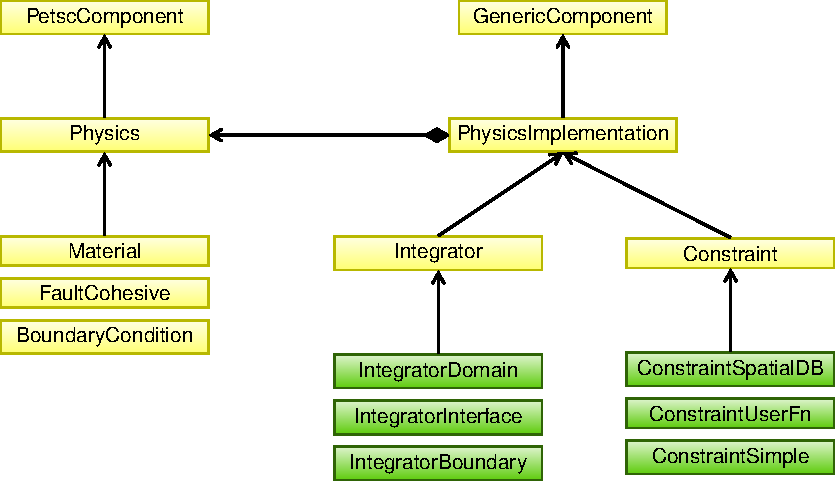
\includegraphics[scale=0.8]{developer/figs/physics_classdiagram}
  \caption{Class diagram for the \object{Physics}.}
  \label{fig:developer:physics:class}
\end{figure}

\subsection{PyLith Application Flow}

The PyLith application driver performs two main functions. First, it
collects all user parameters from input files (e.g., \filename{.cfg}
files) and the command line, and then it performs from simple checks
on the parameters. Second, it launches the MPI job.

Once the MPI job launches, the application flow is:
\begin{enumerate}
\item Read the finite-element mesh; \object{pylith.meshio.MeshImporter}.
  \begin{enumerate}
  \item Read the mesh (serial); \object{pylith::meshio::MeshIO}.
  \item Reorder the mesh; \object{pylith::topology::ReverseCuthillMcKee}.
  \item Insert cohesive cells as necessary (serial); \object{pylith::faults::FaultCohesive}.
  \item Distribute the mesh across processes (parallel); \object{pylith::topology::Distributor}.
  \item Refine the mesh if desired (parallel); \object{pylith::topology::RefineUniform}.
  \end{enumerate}
\item Setup the problem.
  \begin{enumerate}
  \item Preinitialize the problem by passing information from Python
    to C++ and doing minimal setup; \object{pylith.Problem.preinitialize()}.
  \item Perform consistency checks and additional checks of user
    parameters; \object{pylith.Problem.verifyConfiguration()}.
  \item Complete initialization of the problem;
    \object{pylith::problems::Problem::initialize()}.
  \end{enumerate}
\item Run the problem; \object{pylith.problems.Problem.run()}.
\item Cleanup; \object{pylith.problems.Problem.finalize()}.
  \begin{enumerate}
  \item Close output files.
  \item Deallocate memory.
  \item Output PETSc log summary, if desired.
  \end{enumerate}
\end{enumerate}

In the first step, we list the object performing the work, whereas in
subsequent steps we list the top-level object method responsible for
the work. Python objects are listed using the \object{path.class}
syntax while C++ objects are listed using \object{namespace::class}
syntax. Note that a child class may redefine or perform additional
work compared to what is listed in the parent class method.

Reading the mesh and the first two steps of the problem setup are
controlled from Python. That is, at each step Python calls the
corresponding C++ methods using SWIG. Starting with the complete
initialization of the problem, the flow is controlled at the C++
level.

\subsubsection{Time-Dependent Problem}

In a time-dependent problem, the PETSc \object{TS} object (relabeled
\object{PetscTS} within PyLith) controls the time stepping. At the
beginning of each time step, the \object{PetscTS} object calls
\object{problems::TimeDependent::prestep()}, and at the end of each
time step, it calls \object{problems::TimeDependent::poststep()}.
Within each time step, the \object{PetscTS} object calls the PETSc
linear and nonlinear solvers as needed, which call the following
methods of the C++ \object{pylith::problems::TimeDependent} object as
needed
\object{computeRHSResidual()},
\object{computeRHSJacobian()},
\object{computeLHSResidual()}, and
\object{computeLHSJacobian()}.
The \object{pylith::problems::TimeDependent} object calls the corresponding methods in the boundary conditions,
constraints, and materials objects.

\subsubsection{Boundary between Python and C++}

The Python code is limited to collecting user input. Everything else
is done in C++. This facilitates debugging (it is easier to track
symbols in the C/C++ debugger) and unit testing, and reduces the
amount of information that needs to be passed from Python to C++. The
source code that follows shows the essential ingradients for Python
and C++ objects, using the concrete example of the \object{Material}
objects.

\userwarning{The examples below show skeleton Python and C++ objects to illustrate the essential ingredients. We have
ommitted documentation and comments that we would normally include and simplified the object hierarchy. See
Section~\vref{cha:code:style} for  details about the coding style we use in PyLith.}

\important{Consistent inheritance between C++ and Python is important in order for SWIG to generate a Python interface
that is consistent with the C++ interface.}

\begin{python}[Skeleton Python object in PyLith]
rom pylith.utils.PetscComponent import PetscComponent
from .materials import Material as ModuleMaterial

# Python objects should inherit the corresponding SWIG interface object (ModuleMaterial).
# Python object inheritance should match C++ object inheritance.
class Material(PetscComponent, ModuleMaterial):

    # Pyre inventory: properties and facilities
    import pyre.inventory

    materialId = pyre.inventory.int("id", default=0)
    materialId.meta['tip'] = "Material identifier (from mesh generator)."

    label = pyre.inventory.str("label", default="", validator=validateLabel)
    label.meta['tip'] = "Descriptive label for material."


    # Public methods

    def __init__(self, name="material"):
        IntegratorPointwise.__init__(self, name)
        return

    def preinitialize(self, mesh):

        # Create the C++ object. This method must be called exactly once.
        self._createModuleObj()

        # Pass name of Pyre component to C++
        ModuleMaterial.setIdentifier(self, self.aliases[-1])

        # Pass Pyre inventory to C++
        ModuleMaterial.id(self, self.materialId)
        ModuleMaterial.label(self, self.label)
        return

    def verifyConfiguration(self, solution):
        # Avoid implementing this method at the Python level if at all possible.
        return


    # Private methods

    def _createModuleObj(self):
        ModuleMaterial.__init__(self)
        return

\end{python}

\begin{cplusplus}[Skeleton C++ header file in PyLith]
#if !defined(pylith_materials_material_hh) // Include guard
#define pylith_materials_material_hh

#include "materialsfwd.hh" // forward declaration of Material object

#include "pylith/utils/PyreComponent.hh" // ISA PyreComponent

class pylith::materials::Material : public pylith::utils::PyreComponent {
    friend class TestMaterial // unit testing

public: // public methods

    // Constructor and desctructor

    Material(const int dimension);
    virtual ~Material(void);

    // Method to deallocate PETSc data structures before calling PetscFinalize().
    virtual void deallocate(void);

    // Accessors

    int dimension(void) const;
    void id(const int value);
    int id(void) const;
    void label(const char* value);
    const char* label(void) const;

    // Initialization

    void verifyConfiguration(const pylith::topology::Field& solution);
    void initialize(const pylith::topology::Field& solution);

    // Finite-element integration

    void computeRHSResidual(pylith::topology::Field* residual,
                            const PylithReal t,
                            const PylithReal dt,
                            const pylith::topology::Field& solution);
    void computeRHSJacobian(PetscMat jacobianMat,
                            PetscMat preconMat,
                            const PylithReal t,
                            const PylithReal dt,
                            const pylith::topology::Field& solution);


private: // Data members

    const int _dimension;
    int _id;
    std::string _label;

    static const char* _pyreComponent; // Name of Pyre component.


private: // Methods not implemented by design to avoid expensive copies.

    Material(const Material&);
    const Material& operator=(const Material&);

};

#endif // pylith_materials_material_hh
\end{cplusplus}

\begin{cplusplus}[Skeleton C++ definition file in PyLith]
// Information about local configuration generated while running configure script.
#include <portinfo>

#include "Material.hh" // implementation of object methods

pylith::materials::Material::Material(const int dimension) :
     _dimension(dimension),
     _id(0),
     _label("") {
    pylith::utils::PyreComponent::setName("material");
} // constructor

pylith::materials::Material::~Material(void) {
    deallocate();
} // destructor

void
pylith::materials::Material::deallocate(void) {
    PYLITH_METHOD_BEGIN;

    // Deallocate PETSc and other data structures

    PYLITH_METHOD_END;
} // deallocate

int
pylith::materials::Material::dimension(void) const {
    return _dimension;
}

void
pylith::materials::Material::id(const int value) {
    PYLITH_COMPONENT_DEBUG("id(value="<<value<<")");

    _id = value;
} // id

int
pylith::materials::Material::id(void) const {
    return _id;
} // id

void
pylith::materials::Material::label(const char* value) {
    PYLITH_COMPONENT_DEBUG("label(value="<<value<<")");

    _label = value;
} // label

const char*
pylith::materials::Material::label(void) const {
    return _label.c_str();
} // label

void
pylith::materials::Material::initialize(const pylith::topology::Field& solution) {
    PYLITH_METHOD_BEGIN;
    PYLITH_COMPONENT_DEBUG("intialize(solution="<<solution.getLabel()<<")");

    // Implementation not shown.

    PYLITH_METHOD_END;
} // initialize

// Implementation of other methods not shown.

\end{cplusplus}


\subsubsection{SWIG Interface Files}

SWIG interface files are essentially stripped down versions of C++ header files. Because SWIG only implements the public
interface, we omit all data members and all protected and private data methods that are not abstract methods or
implement abstract methods.

\begin{cplusplus}[SWIG interface file]
// The class declaration must appear within the appropriate namespace blocks.

namespace pylith {
    namespace materials {

        class Material : public pylith::utils::PyreComponent {
            public: // public methods

            // Constructor and desctructor

            Material(const int dimension);
            virtual ~Material(void);

            // Method to deallocate PETSc data structures before calling PetscFinalize().
            virtual void deallocate(void);

            // Accessors

            int dimension(void) const;
            void id(const int value);
            int id(void) const;
            void label(const char* value);
            const char* label(void) const;

            // Initialization

            void verifyConfiguration(const pylith::topology::Field& solution);
            void initialize(const pylith::topology::Field& solution);

            // Finite-element integration

            void computeRHSResidual(pylith::topology::Field* residual,
                                    const PylithReal t,
                                    const PylithReal dt,
                                    const pylith::topology::Field& solution);
            void computeRHSJacobian(PetscMat jacobianMat,
                                    PetscMat preconMat,
                                    const PylithReal t,
                                    const PylithReal dt,
                                    const pylith::topology::Field& solution);

        };
    }
}

\end{cplusplus}


% End of file
